\documentclass[paper=a4, fontsize=9pt]{scrartcl}
\usepackage[bottom=0.9in, left=0.7in, right=0.7in, top=0.8in, foot=0.5in]{geometry}
\usepackage{layouts}

\usepackage[usenames,dvipsnames,x11names]{xcolor}

\usepackage[T1]{fontenc}
\usepackage{fourier}
\usepackage[english]{babel}
\usepackage{amsmath,amsfonts,amsthm}

\usepackage{sectsty}
\allsectionsfont{\centering \normalfont\scshape}

\usepackage{amssymb}
\usepackage{acronym}
\usepackage{booktabs}
\usepackage{caption}
\usepackage{fancyhdr}
\usepackage{float}
\usepackage{graphicx}
\usepackage[htt]{hyphenat}
\usepackage{lastpage}
\usepackage{multicol}
\usepackage{titlesec}
\usepackage[inline]{enumitem}
\usepackage{algorithm, algpseudocode}
\usepackage[export]{adjustbox}
\usepackage{pdflscape}

\usepackage{tikz}
\usepackage{pgfplots, pgfplotstable}
\pgfplotsset{compat=1.5}
\usepgfplotslibrary{colorbrewer}

\pagestyle{fancyplain}
\fancyhead{}
\fancyfoot[L]{}
\fancyfoot[C]{\thepage~of~4}
\renewcommand{\headrulewidth}{0pt}
\renewcommand{\footrulewidth}{0pt}
\setlength{\headheight}{13.6pt}

\newcommand{\horrule}[1]{\rule{\linewidth}{#1}}

\title{
\vspace{-1cm}
\normalfont \normalsize
\textsc{Norwegian University of Science and Technology\\IT3708 -- Bio-Inspired Artificial Intelligence}
\horrule{0.5pt} \\[0cm]
\Huge Project 4: Solving Job Shop Scheduling Problem\\Using Bio-Inspired Algorithms\\[-0.3cm]
\horrule{2pt} \\[0.1cm]
}

\newacro{JSSP}{Job-Shop Scheduling Problem}
\newacro{ACO}{Ant Colony Optimization}
\newacro{BA}{Bees Algorithm}
\newacro{PSO}{Particle Swarm Optimization}
\newacro{TS}{Taboo Search}

\author{Per Magnus Veierland\\permve@stud.ntnu.no}

\date{\normalsize\today}

\begin{document}

\maketitle

\setlength\columnsep{20pt}

\begin{multicols}{2}

% TODO Explain how schedules are built from solutions

% Representation of solutions (individual & chromosome) for each of the three algorithm representations. Using figure(s) for solution is a must. For each of the three algorithms, how do you build the schedule from respective solutions? (1.5p)

\section*{Schedule Representation}

All three optimizers utilize the same schedule representation as shown in Figure~\ref{figure:representation}. This representation is able to represent both infeasible and feasible solutions to the \ac{JSSP}. Depending on context in the implementation, this representation either represents the job preference for each machine in a solution, or it represents a solution to the \ac{JSSP} directly. For both the \ac{PSO} and the \ac{BA}, random individuals are generated as part of the search. This is done by building a schedule with a randomly permuted job ordering for each machine. If treated as a solution directly, such a solution may be infeasible as machines can deadlock. To ensure that all created solutions are feasible, each possibly infeasible solution is ``developed'' by treating the representation as a preference description. The G\&T~algorithm as described in \cite{sha2006hybrid} details how a preference description can be used to generate an active schedule which must be feasible.

The G\&T algorithm can be described in four steps:

\begin{enumerate}
    \item Initialize schedule $S=\varnothing$; $\Omega$ is initialized to contain all operations without job predecessors.
    \item Find $o^*=\arg \min_{o \in \Omega} f_o$, where $f_o$ is the earliest completion time for operation $o$; $f_o = s_o + p_o$, where $s_o$ is the earliest starting time for operation $o$, and $p_o$ is the processing time for operation $o$.
    \item \begin{enumerate}
        \item Identify conflict set $C = \{ o \in \Omega \vert m_o = m_{o^*} \land s_o < f_{o^*} \}$, where $m_o$ is the machine associated with $o$.
        \item Select $o \in C$ according to the preference specified in the encoded representation.
        \item Add $o$ to schedule $S$.
    \end{enumerate}
    \item If schedule $S$ is incomplete; remove $o$ from $\Omega$ and add its immediate job successor to $\Omega$ and continue from step~2.
\end{enumerate}

{
\vspace{0.3cm}
\centering
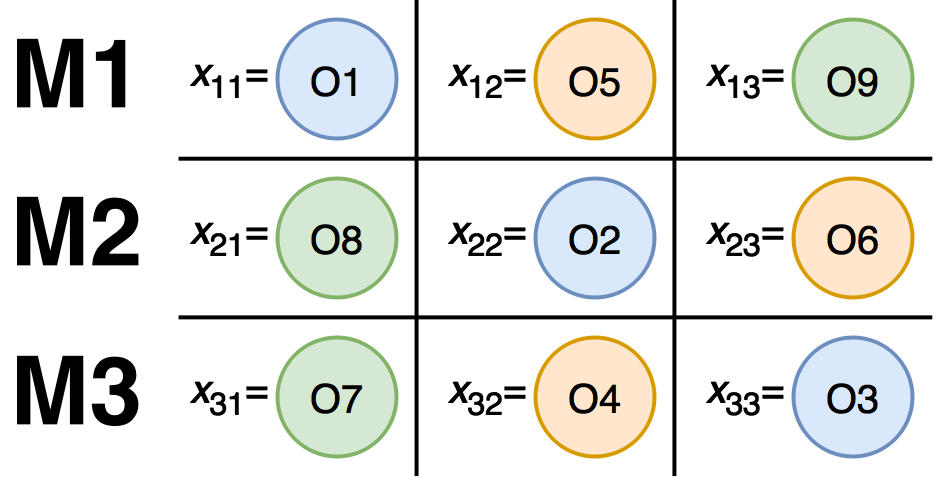
\includegraphics[scale=0.2]{figures/permve-ntnu-it3708-project-4-2017-schedule-representation}
\captionof{figure}{A \acs{JSSP} schedule is represented as an $m \times n$ matrix of $m$ machines and $n$ jobs. \textcolor{NavyBlue}{$\text{Job~1} = \langle\,\text{O1}, \text{O2}, \text{O3}\,\rangle$}, \textcolor{Melon}{$\text{Job~2} = \langle\,\text{O4}, \text{O5}, \text{O6}\rangle$}, \textcolor{OliveGreen}{$\text{Job~3} = \langle \text{O7}, \text{O8}, \text{O9}\rangle$}. Each row $i$ encodes the ordering of operations for machine $i$; M1, M2, M3.}
\label{figure:representation}
\vspace{0.3cm}
}

\section*{\acl{PSO}}

% TODO Figure explaining PSO representation

\section*{\acl{ACO}}

% TODO Figure explaining ACO representation

\section*{\acl{BA}}

% TODO Figure explaining BA representation

\section*{\acl{TS}}

\bibliographystyle{unsrt}
\bibliography{references.bib}

{
\begin{minipage}{\linewidth{}}
\centering
\begin{tabular}{lc}
\toprule
Parameter                                   & Value \\
\midrule
Iterations                                  & 150   \\
Swarm size                                  & 100   \\
Particle best factor ($c_1$)                &   0.5 \\
Global best factor ($c_2$)                  &   0.3 \\
Probability of not resetting velocity ($w$) &   0.5 \\
\bottomrule
\end{tabular}
\captionof{table}{\acf{PSO} parameters.}
\label{table:psoparams}
\end{minipage}
}

{
\begin{minipage}{\linewidth{}}
\centering
\begin{tabular}{lc}
\toprule
Parameter                                         & Value \\
\midrule
Iterations                                        & 20    \\
Heuristic power ($\beta$)                         & 10.0  \\
Evaporation rate ($\rho$)                         &  0.1  \\
Initial pheromone value ($\tau_{\text{initial}}$) &  0.5  \\
\bottomrule
\end{tabular}
\captionof{table}{\acf{ACO} parameters.}
\label{table:acoparams}
\end{minipage}
}

{
\begin{minipage}{\linewidth{}}
\centering
\begin{tabular}{lc}
\toprule
Parameter                              & Value \\
\midrule
Iterations                             &  5 \\
Number of scouts ($n$)                 & 10 \\
Number of sites selected ($m$)         &  8 \\
Number of elite sites ($e$)            &  3 \\
Number of normal sites ($m-e$)         &  5 \\
Number of bees per elite site ($nep$)  &  1 \\
Number of bees per normal site ($nsp$) &  2 \\
\bottomrule
\end{tabular}
\captionof{table}{\acf{BA} parameters.}
\label{table:baparams}
\end{minipage}
}

{
\begin{minipage}{\linewidth{}}
\centering
\begin{tabular}{lc}
\toprule
Parameter                                             & Value \\
\midrule
Iteration limit (maxiter)                             &   150 \\
Total iteration limit ($\text{maxiter}_\text{total}$) &  1000 \\
Taboo list limit (maxt)                               &     5 \\
Backtracking limit (maxl)                             &     8 \\
Max cycle detection count ($\max c$)                  &     2 \\
Max cycle detection duration ($\max \delta$)          &   100 \\
\bottomrule
\end{tabular}
\captionof{table}{\acf{TS} parameters.}
\label{table:tsparams}
\end{minipage}
}

\end{multicols}

%\clearpage

% TODO Explain local search + figure

% For test problem #3, draw the gantt-chart targeting the best makespan. You need to draw for all three algorithms. (1.5p)

% \begin{landscape}
% {
% \begin{table}
% \hspace*{-0.5cm}
% \centering
% \begin{tabular}{l}
% 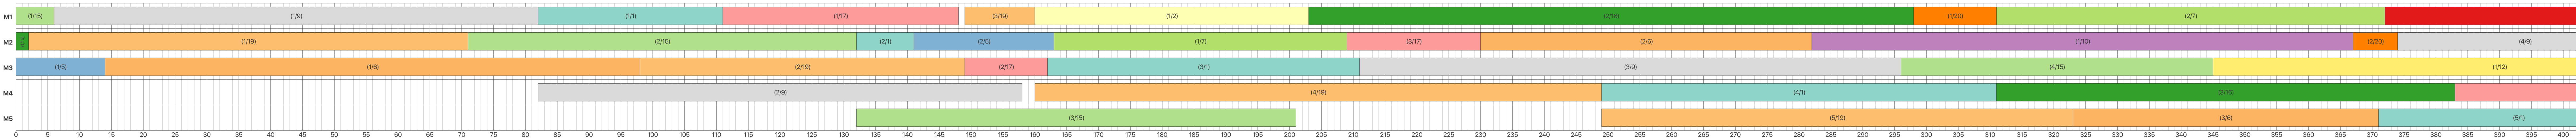
\includegraphics[height=40pt]{figures/solution_pso_instance_3_1_scaled}\\[0.15cm]
% \hspace{0.90909pt}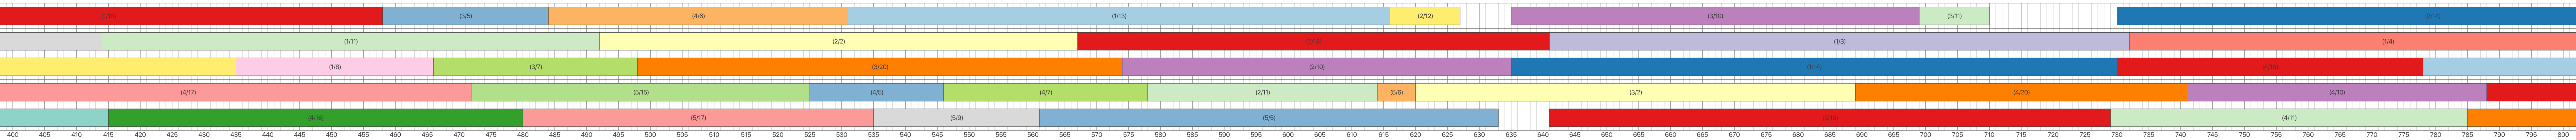
\includegraphics[height=40pt]{figures/solution_pso_instance_3_2_scaled}\\[0.15cm]
% \hspace{0.90909pt}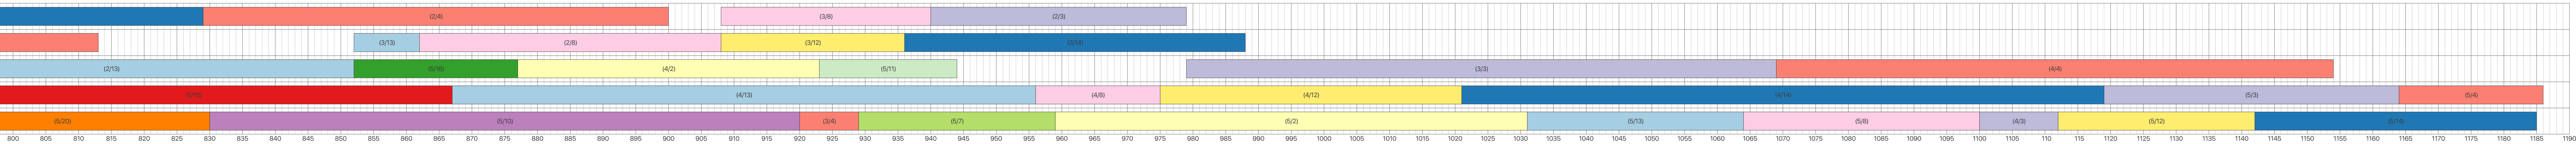
\includegraphics[height=40pt]{figures/solution_pso_instance_3_3_scaled}\\
% \multicolumn{1}{c}{\textit{Figure 1: \acf{PSO} solution with makespan 1186 for problem~3 using parameters specified in Table~\ref{table:psoparams}~and~\ref{table:tsparams}.}}\\[1.2cm]
% 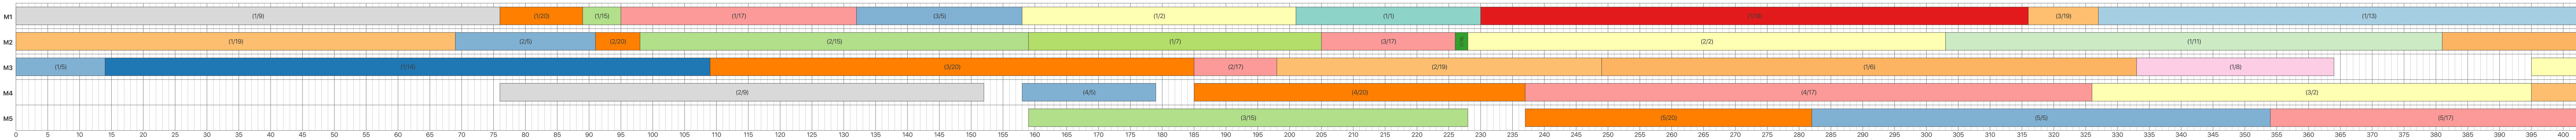
\includegraphics[height=40pt]{figures/solution_aco_instance_3_1_scaled}\\[0.15cm]
% \hspace{0.90909pt}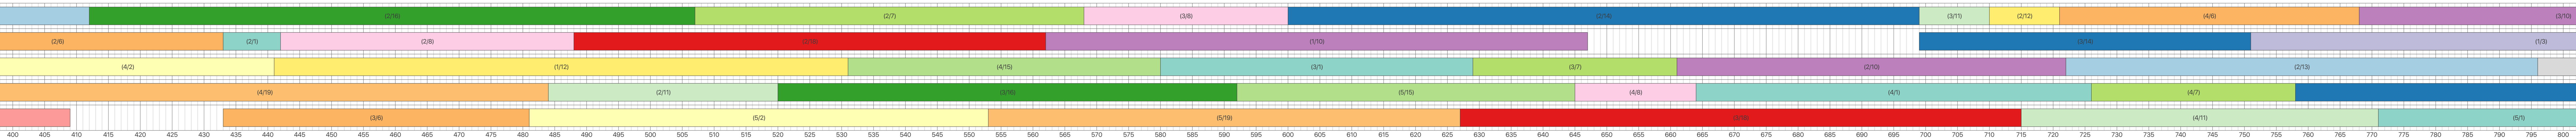
\includegraphics[height=40pt]{figures/solution_aco_instance_3_2_scaled}\\[0.15cm]
% \hspace{0.90909pt}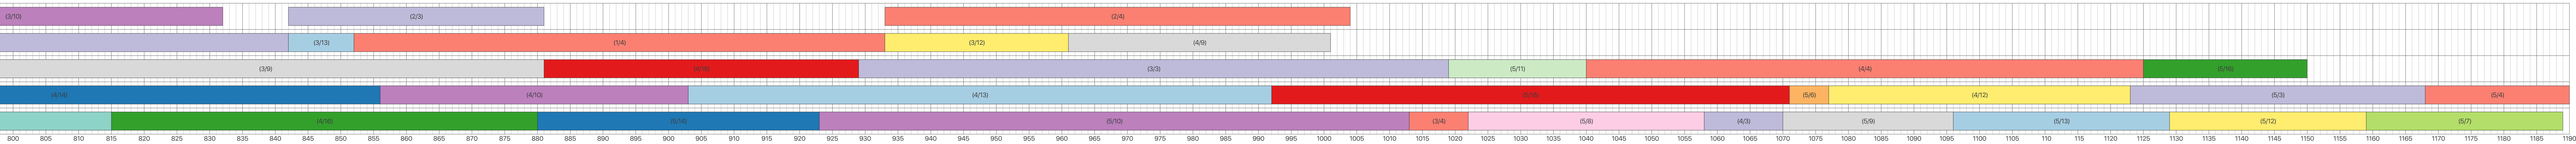
\includegraphics[height=40pt]{figures/solution_aco_instance_3_3_scaled}\\
% \multicolumn{1}{c}{\textit{Figure 2: \acf{ACO} solution with makespan 1190 for problem~3 using parameters specified in Table~\ref{table:acoparams}~and~\ref{table:tsparams}.}}\\[1.2cm]
% 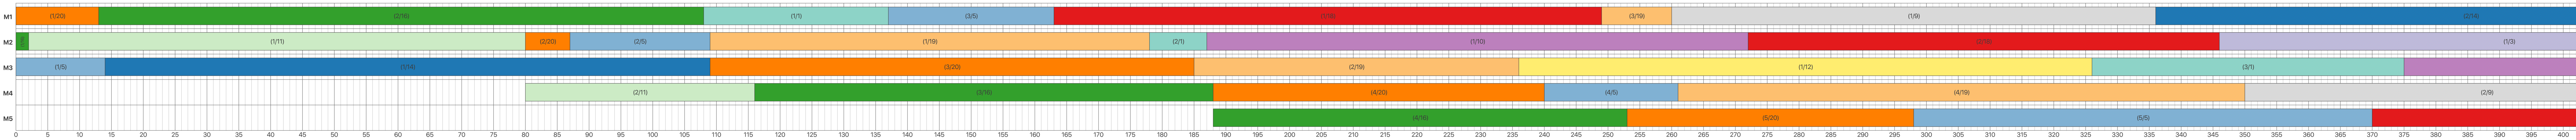
\includegraphics[height=40pt]{figures/solution_ba_instance_3_1_scaled}\\[0.15cm]
% \hspace{0.90909pt}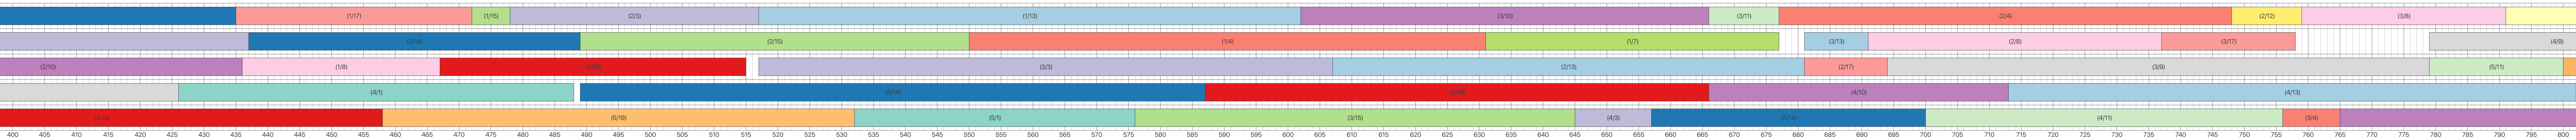
\includegraphics[height=40pt]{figures/solution_ba_instance_3_2_scaled}\\[0.15cm]
% \hspace{0.90909pt}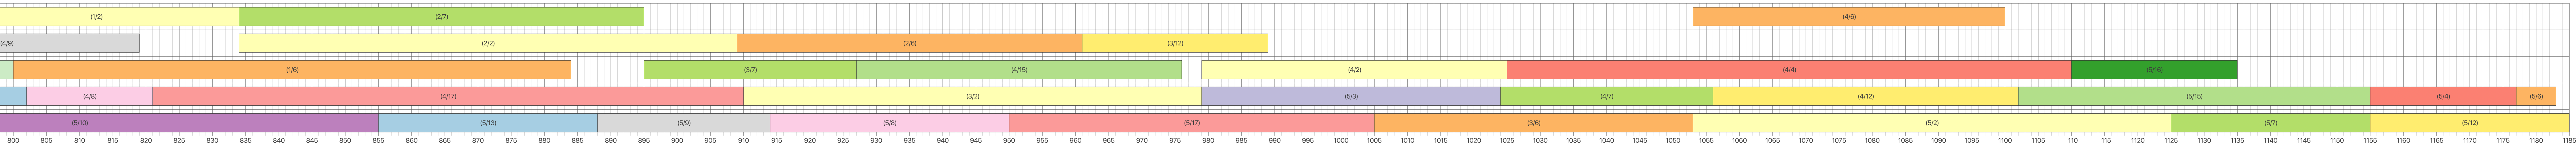
\includegraphics[height=40pt]{figures/solution_ba_instance_3_3_scaled}\\
% \multicolumn{1}{c}{\textit{Figure 3: \acf{BA} solution with makespan 1185 for problem~3 using parameters specified in Table~\ref{table:baparams}~and~\ref{table:tsparams}.}}\\
% \end{tabular}
% \end{table}
% }
% \end{landscape}

\end{document}
